%%%
%
% $Autor: Wings $
% $Datum: 2021-05-14 $
% $Pfad: GitLab/CornerBlending $
% $Dateiname: ArcStrategy
% $Version: 4620 $
%
% !TeX spellcheck = de_GB
%
%%%


\chapter{Datasets}
\label{Datasets}
\section{Charactaristics of the dataset}
For our project to be successful, the dataset we use must adhere to certain criteria. Firstly, the data must be numerical in nature and correspond to the output of an Inertial Measurement Unit (IMU). This is crucial for the efficient processing of the data by the algorithm and subsequent recording by our device.

Secondly, we have a specific set of locomotion types that need to be analyzed, including walking, running, sitting, standing, or in other words normal daily activities performed by an office worker.

Finally, having a sufficient amount of data is vital for us to make accurate estimations of daily activities. This highlights the importance of collecting a robust dataset that can support our analysis.

Furthermore, there have been various studies and research initiatives that have focused on human locomotion recognition, providing datasets that are accessible for use. Out of these, three datasets that have utilized wearable Inertial Measurement Unit (IMU) sensors have particularly piqued my interest. These datasets demonstrate the feasibility of using wearable IMU sensors for human locomotion recognition, providing valuable insights that can inform our project.
\section{The Wireless Sensor Data Mining Dataset }
includes IMU data collected from smartphones worn by participants during various activities, including Walking, Jogging, Upstairs, Downstairs, Sitting, Standing. 
\subsection{Relevant information}

The WISDM (Wireless Sensor Data Mining) dataset is a collection of data related to human activity recognition, captured using cell phone accelerometers. It was released by the WISDM Lab  <http://www.cis.fordham.edu/wisdm/> at Fordham University, as part of their research efforts in the field, as published in the paper ``Activity Recognition using Cell Phone Accelerometers'' in the Proceedings of the Fourth International Workshop on Knowledge Discovery from Sensor Data (KDD-10) held in Washington D.C. in 2010. \cite{Kwapisz:2010}

The WISDM (Wireless Sensor Data Mining) dataset comes with five files, \FILE{readme.txt}, 

\medskip

\FILE{WISDM\_ar\_v1.1\_raw\_about.txt}

 \medskip

 \FILE{WISDM\_ar\_v1.1\_trans\_about.txt}
 \medskip
 
\FILE{WISDM\_ar\_v1.1\_raw.txt}
\medskip

 \FILE{WISDM\_ar\_v1.1\_transformed.arff}
 
These files provide us with raw data, transformed data and the needed information about them: 

The raw data includes 1,098,207 examples, each with 6 attributes and no missing values. The classification tasks associated with this dataset include walking, jogging, upstairs, downstairs, sitting, and standing, with a class distribution of 38.6\% for walking, 31.2\% for jogging, 11.2\% for upstairs, 9.1\% for downstairs, 5.5\% for sitting, and 4.4\% for standing.

	
The raw data is stored in a file named \FILE{WISDM\_ar\_v1.1\_raw.txt} and follows the format


\medskip

 \PYTHON{\footnotesize [user],[activity],[timestamp],[x-acceleration],[y-acceleration],[z-acceleration];}
 
\medskip

A representative example of the data is: 

\medskip

\PYTHON{33,Jogging,49105962326000,-0.6946377,12.680544,0.50395286;}

\medskip
 
The sampling rate for the data collection was 20Hz, meaning one sample was collected every 50ms. The dataset comes with a readme file that provides additional information on the WISDM Lab, rights and permissions, raw and transformed data, and more detailed information on the class distribution, data format, and sampling rate. (zitieren) 

the Activity Recognition using Cell Phone Accelerometers study by Kwapisz that created the database works with standard classification algorithms which cannot be directly applied to raw time-series accelerometer data. \cite{Weiss:1998} Instead, they first had to tranformed the raw time series data into examples. 
in 2.2 \cite{Kwapisz:2010} its is explained that they divided the data into 10-second segments and then generated features that were based on the 200 readings contained within each 10-second segment. they refer to the duration of each segment as the example duration (ED).  10-second ED has proven to providsufficient time to capture several repetitions of the (repetitive) motions involved in some of the six activities. 
The transformed data includes 5,424 with 46 attributes and no missing attribute values.
The distribution of classes is as follows:

Walking -> 2,082 -> 38.4\%,

Jogging -> 1,626 -> 30.0\%,

Upstairs -> 633 -> 11.7\%,

Downstairs -> 529 -> 9.8\%,

Sitting -> 307 -> 5.7\%,

Standing -> 247 -> 4.6\% 


\subsection{Advantages and Limitations of the WISDM Dataset for Human Activity Recognition}
\textbf{Accuracy:} 
The study conducted in \cite{Kwapisz:2010} employed three classification techniques from the WEKA data mining suite to predict user activities, including decision trees (J48), logistic regression, and multilayer neural networks. Results from the study, as demonstrated in \ref{Table: Accuracies of Activity Recognition}, show that high levels of accuracy were achieved in most cases. For the two most common activities of walking and jogging, all three learning algorithms achieved accuracy levels above 89.9\% and 96.5\% respectively. Furthermore, the accuracy for sitting was 92.2\% and for standing was over 87\%.
\begin{figure}
	\centering
	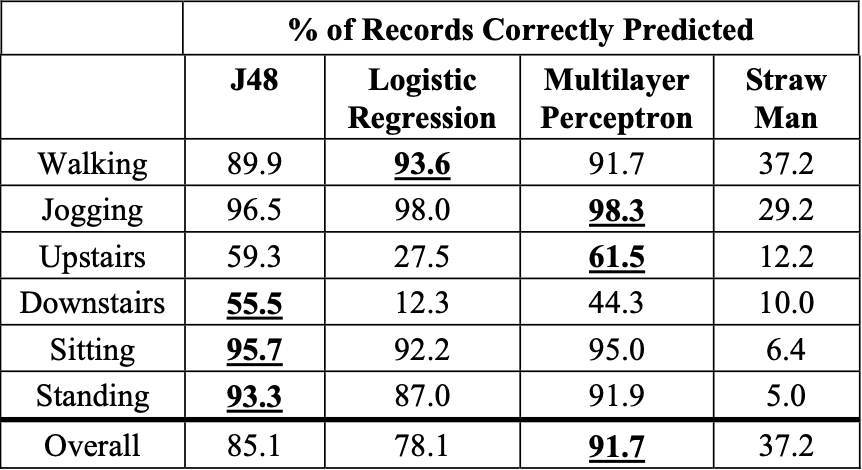
\includegraphics[width=0.5\textwidth]{Images/Table Accuracies of Activity Recognition}
	\caption{Accuracies of Activity Recognition.\cite{Kwapisz:2010}}
	\label{Table: Accuracies of Activity Recognition}
\end{figure}


\textbf{Relevance:} 
For the purpose of our study, we require the classification of four types of movements: walking, running, sitting, and standing. The WISDM dataset provides data relevant to these movements, thereby eliminating the need to collect additional data.

\textbf{Unbalanced:} 
The WISDM dataset aims to classify human activity, but its target variable has an unbalanced distribution. According to the "raw\_about.txt" file that comes with the dataset, walking accounts for 38.6\% of the activities, jogging for 31.2\%, upstairs for 11.2\%, downstairs for 9.1\%, sitting for 5.5\%, and standing for 4.4\%. This disparity in the distribution of activities is clearly shown in the dataset.

\textbf{Unbalanced:} 
%we only have data from the accelometer 

\section{The UCI Human Activity Recognition dataset}
The UCI Human Activity Recognition dataset was created from recordings of 30 individuals as they performed daily activities while wearing a waist-mounted smartphone with integrated inertial sensors.

\subsection{Relevant information}
 
 The 30 volunteers, ranging in age from 19 to 48 years old, carried out six activities including walking, walking upstairs, walking downstairs, sitting, standing, and laying \ref{Activity Recognition process pipeline}. For each activity, data was collected at a constant rate of 50Hz  on three-axis acceleration from the accelerometer, three-axis angular velocity from the gyroscope and a 561-feature vector that includes time and frequency domain variables. This information, along with the activity label and the participant's identifier, was recorded in the database.
 In total, the dataset contains 10,299 entries and 563 features. The aim of the study was to classify the activities performed into one of the six categories. The data was recorded and labeled through video recording. The obtained dataset was randomly divided into two sets, with 70\% of the volunteers being used to generate training data and 30\% for testing data.
 
 \begin{figure}
 	\centering
 	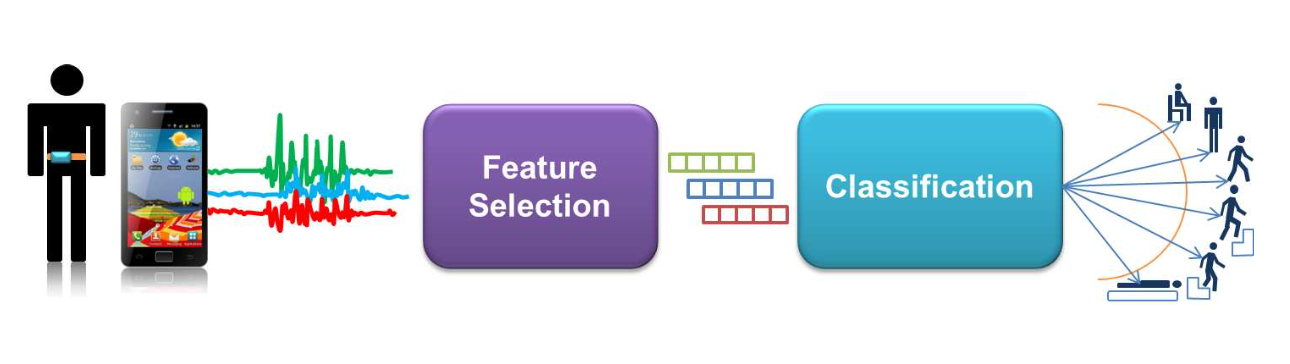
\includegraphics[width=1\textwidth]{Images/Activity Recognition process pipeline}
 	\caption{UCI Human Activity Recognition process pipeline \cite{Anguita:2012}}
 	\label{Activity Recognition process pipeline}
 \end{figure}
%https://www.youtube.com/watch?v=GN9x2F_OQQM&t=32s&ab_channel=sukruthh1
 %\cite{Anguita:2012} 
\subsection{Advantages and Limitations of the UCI Human Activity Recognition dataset}

\textbf{Multiple Sensor Modalities:} The UCI Human Activity Recognition dataset includes data from multiple sensor sources, such as accelerometers and gyroscopes, providing a more comprehensive representation of human activities.

%\textbf{Well-known and Widely Used:} The UCI Human Activity Recognition dataset is a commonly recognized and utilized resource for the development and evaluation of human activity recognition models.

\textbf{Balanced Dataset:}

\textbf{Limited Activity Types:} The UCI Human Activity Recognition dataset only includes six types of activities, and does not include "jogging", which requires additional self-recording to be included in the analysis.

\textbf{Small Sample Size:} The UCI Human Activity Recognition dataset is relatively small and only includes data from 30 subjects, potentially limiting its ability to generalize to a larger population or additional activities.

\textbf{Controlled Data Collection:} The UCI Human Activity Recognition dataset was collected using a specific protocol in controlled environments, which may not reflect real-world scenarios. This could impact the generalizability of models developed from this data to real-world human activity recognition problems.


\section{The OPPORTUNITY++ dataset}
\subsection{Relevant information}

The OPPORTUNITY Dataset is a comprehensive collection of data for human activity recognition obtained from wearable, object, and ambient sensors. The purpose of the dataset is to evaluate and compare algorithms for activity recognition, including classification, data segmentation, sensor fusion, and feature extraction. A part of the OPPORTUNITY dataset was utilized in the OPPORTUNITY Activity Recognition Challenge held during the 2011 IEEE International Conference on Systems, Man, and Cybernetics Workshop. \cite{Chavarriaga:2011} 

The dataset was collected from 12 participants during their morning activities and includes 72 sensors from 10 different modalities across 15 wireless and wired sensor systems in the environment, objects, and on the body (as shown in \ref{Recording environment of the Opportunity dataset} ). Each participant has five daily activity sessions and a drill session with around 20 repetitions of specific actions. The data was labeled manually for modes of movement, gestures, and high-level activities by at least two individuals. The dataset includes the following features:
 \begin{figure}
	\centering
	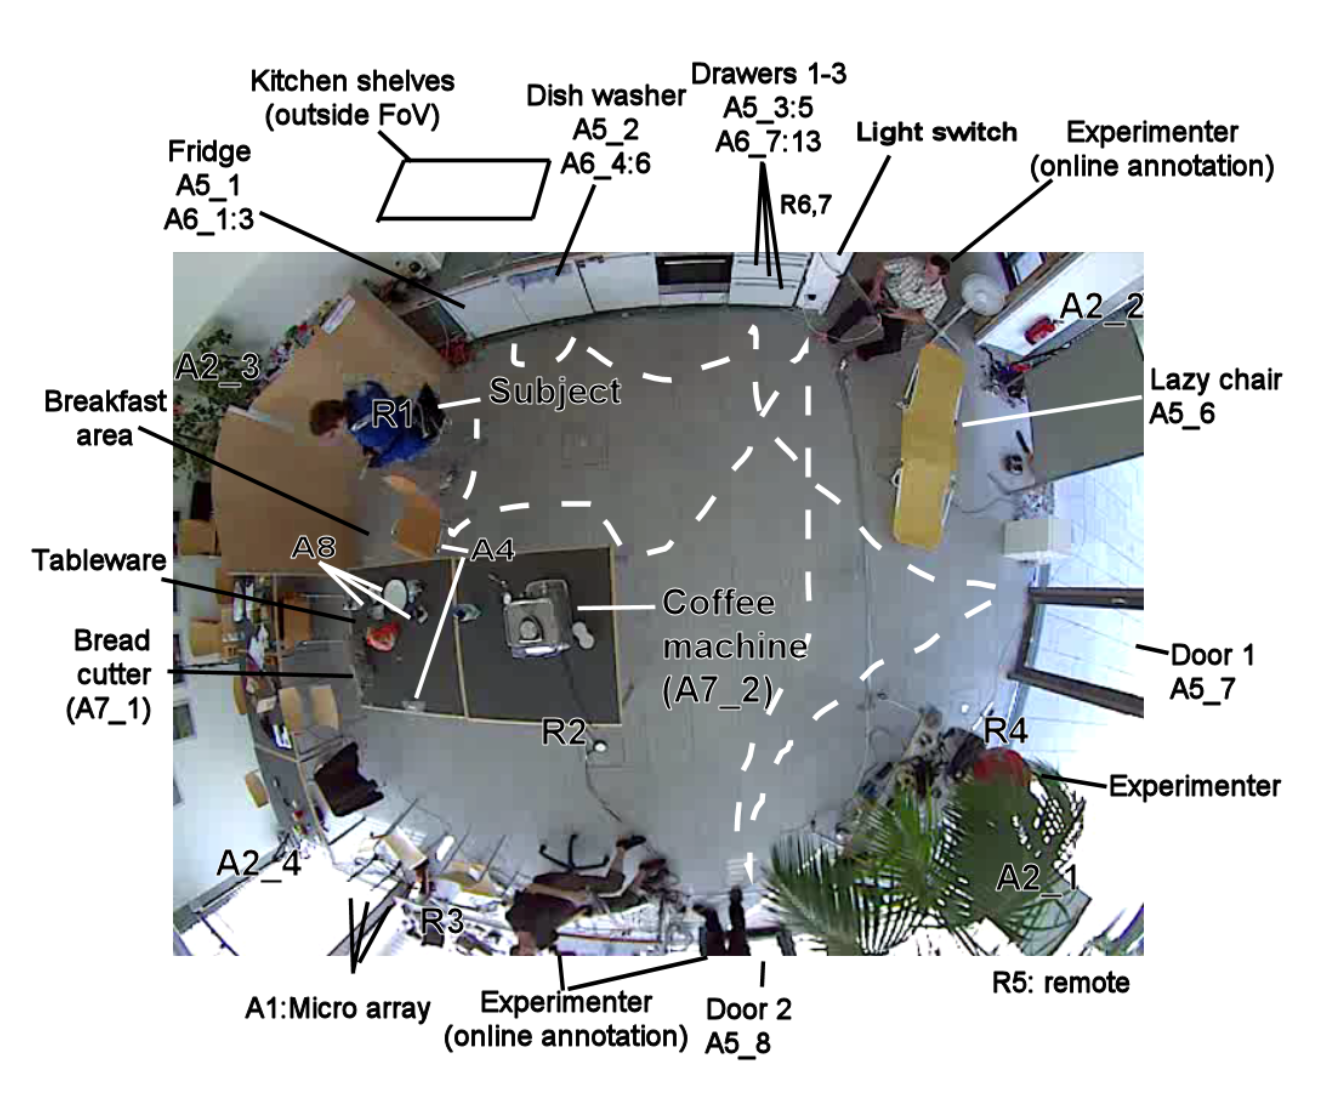
\includegraphics[width=1\textwidth]{Images/Recording environment of the Opportunity dataset}
	\caption{Recording environment of the Opportunity dataset.}\cite{Sagha:2011}
	\label{Recording environment of the Opportunity dataset}
\end{figure}

The OPPORTUNITY dataset consists of sensor readings collected during typical daily activities and includes:

- Body-worn sensors: 7 inertial measurement units, 12 3D acceleration sensors, and 4 3D localization sensors.

- Object sensors: 12 objects equipped with 3D acceleration and 2D rate of turn sensors.

- Ambient sensors: 13 switches and 8 3D acceleration sensors.

- Recordings: 4 participants, each with 6 recorded runs. 5 of these are "Activity of Daily Living" runs representing natural execution of daily activities, while the 6th run is a scripted "drill" run.

- Annotations/Classes: The activities performed by the participants are annotated on various levels, including "modes of locomotion," low-level actions (relating 13 actions to 23 objects), 17 mid-level gesture classes, and 5 high-level activity classes.


The format of the data are numerical Labeled recordings from the sensor used. The label legend contains a unique index and a track name, which are followed by a label name.

 The label columns contain information about the different levels of activities that are annotated for each recording, such as "Locomotion", "HL\_Activity" (high-level activity), "LL\_Left\_Arm" (low-level left arm), "LL\_Left\_Arm\_Object" (object associated with the low-level left arm), "LL\_Right\_Arm" (low-level right arm), "LL\_Right\_Arm\_Object" (object associated with the low-level right arm), and "ML\_Both\_Arms" (mid-level both arms). 

Each column provides information about a specific aspect of the activity that is being performed, with different columns representing different levels of detail about the activity. \cite{Roggen:2010} 
\subsection{Advantages and Limitations of the OPPORTUNITY++ dataset}

The Opportunity dataset has been used in several studies. However, it may not be as suitable for our project for the following reasons:

\textbf{Modality:} The Opportunity dataset is based on wearable sensors that use multiple modalities, including accelerometer, gyroscope, magnetometer, and pressure sensors. This provides a more comprehensive view of human activity, but it may not align with the criteria we have for our project, which requires data from only the Inertial Measurement Unit (IMU).

\textbf{Data Format:}  The Opportunity dataset has a different data format compared to the WISDM dataset. It includes multiple channels of data, making it challenging to integrate it into our project without significant processing.

In conclusion, while the Opportunity dataset may have its strengths, it may not be as well-suited for our project as the WISDM dataset.

\section{Conclusion}
The WISDM dataset is well-suited for human activity recognition due to its numerical data corresponding to the output of an Inertial Measurement Unit (IMU), a sufficient amount of data, and relevance to our analysis of daily activities such as walking, running, sitting, and standing. The study in 2010 achieved high accuracy in activity recognition, with accuracy levels above 89.9\% for walking and 96.5\% for jogging. The dataset has an unbalanced distribution of activities, with walking accounting for 38.6\% and jogging for 31.2\%. The only limitation of the WISDM dataset is that it only includes data from the accelerometer.

